\documentclass[border=6pt]{standalone}
\usepackage[T1]{fontenc}
\usepackage{lmodern}
\usepackage{tikz}
\usetikzlibrary{arrows.meta,positioning,shapes.geometric,calc,fit}
\begin{document}
\hyphenpenalty=10000 \exhyphenpenalty=10000
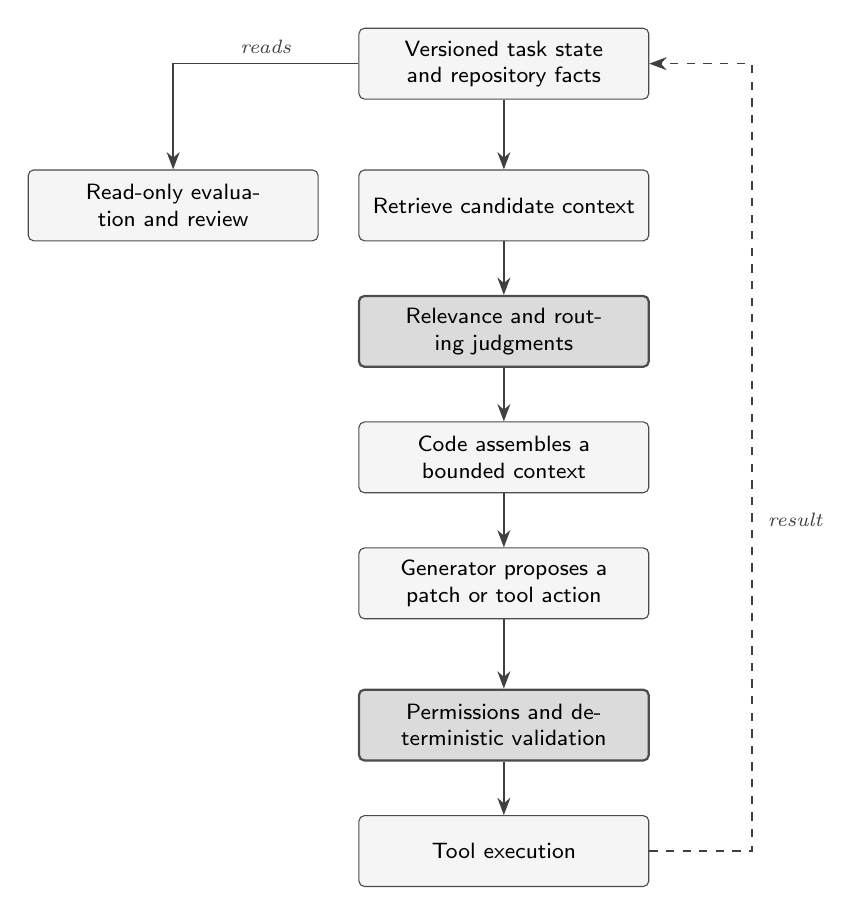
\begin{tikzpicture}[
  font=\footnotesize\sffamily,
  box/.style={draw=black!70, rounded corners=2pt, fill=black!4, align=center,
              text width=3.4cm, minimum height=0.9cm, inner sep=4pt},
  key/.style={box, fill=black!14, line width=0.8pt},
  arr/.style={-{Stealth[length=2.2mm]}, draw=black!75, line width=0.6pt},
  lab/.style={font=\scriptsize\itshape, text=black!75}
]
\node[box] (s) at (0,0) {Versioned task state and repository facts};
\node[box] (k) at (0,-1.8) {Retrieve candidate context};
\node[key] (d) at (0,-3.4) {Relevance and routing judgments};
\node[box] (b) at (0,-5.0) {Code assembles a bounded context};
\node[box] (l) at (0,-6.6) {Generator proposes a patch or tool action};
\node[key] (p) at (0,-8.4) {Permissions and deterministic validation};
\node[box] (x) at (0,-10.0) {Tool execution};
\node[box] (o) at (-4.2,-1.8) {Read-only evaluation and review};

\draw[arr] (s) -- (k);
\draw[arr] (k) -- (d);
\draw[arr] (d) -- (b);
\draw[arr] (b) -- (l);
\draw[arr] (l) -- (p);
\draw[arr] (p) -- (x);
\draw[arr, dashed] (x.east) -- ++(1.3,0) |- (s.east) node[lab, above, pos=0.2, xshift=0.55cm] {result};
\draw[arr] (s.west) -| (o.north) node[lab, above, pos=0.25] {reads};
\end{tikzpicture}
\end{document}
